

\tikzset{every picture/.style={line width=0.75pt}} %set default line width to 0.75pt        

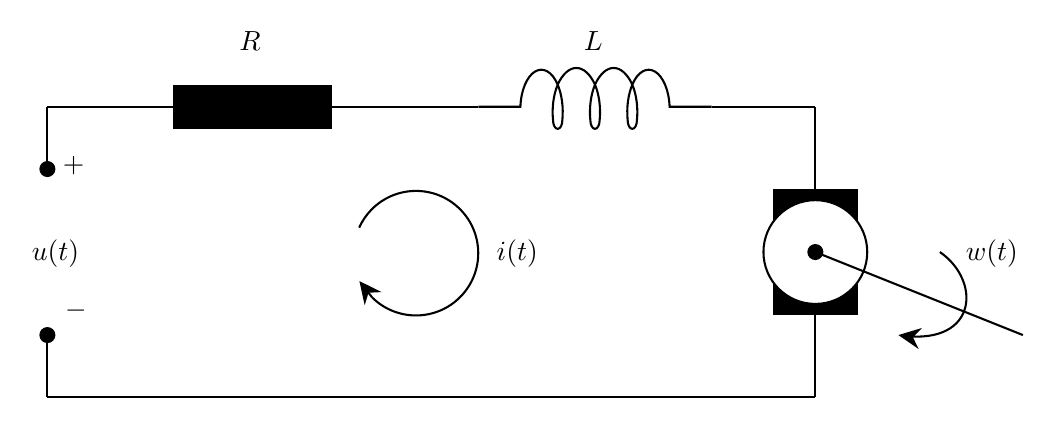
\begin{tikzpicture}[x=0.75pt,y=0.75pt,yscale=-1,xscale=1]
%uncomment if require: \path (0,300); %set diagram left start at 0, and has height of 300

%Shape: Resistor [id:dp759021563450837] 
\draw  [fill={rgb, 255:red, 0; green, 0; blue, 0 }  ,fill opacity=1 ][line width=0.75]  (101.18,100) -- (176.49,100) -- (176.49,120) -- (101.18,120) -- (101.18,100) -- cycle (80,110) -- (101.18,110) (176.49,110) -- (197.67,110) ;
%Straight Lines [id:da9833480980865364] 
\draw [line width=0.75]    (80,110) -- (40,110) ;
%Straight Lines [id:da7530411059484647] 
\draw [line width=0.75]    (40,110) -- (40,140) ;
\draw [shift={(40,140)}, rotate = 90] [color={rgb, 255:red, 0; green, 0; blue, 0 }  ][fill={rgb, 255:red, 0; green, 0; blue, 0 }  ][line width=0.75]      (0, 0) circle [x radius= 3.35, y radius= 3.35]   ;
%Straight Lines [id:da4394842288276831] 
\draw [line width=0.75]    (197.67,110) -- (247.67,110) ;
%Shape: Inductor (Air Core) [id:dp1789049029135794] 
\draw  [line width=0.75]  (247.67,110) -- (267.89,110) .. controls (268.18,102.12) and (270.98,95.38) .. (274.96,93.03) .. controls (278.93,90.67) and (283.26,93.18) .. (285.86,99.34) .. controls (287.87,104.15) and (288.69,110.36) .. (288.11,116.4) .. controls (288.11,118.75) and (287.1,120.66) .. (285.86,120.66) .. controls (284.62,120.66) and (283.61,118.75) .. (283.61,116.4) .. controls (283.03,110.36) and (283.85,104.15) .. (285.86,99.34) .. controls (288.19,94.22) and (291.45,91.31) .. (294.85,91.31) .. controls (298.25,91.31) and (301.5,94.22) .. (303.83,99.34) .. controls (305.84,104.15) and (306.66,110.36) .. (306.08,116.4) .. controls (306.08,118.75) and (305.07,120.66) .. (303.83,120.66) .. controls (302.59,120.66) and (301.59,118.75) .. (301.59,116.4) .. controls (301.01,110.36) and (301.83,104.15) .. (303.83,99.34) .. controls (306.17,94.22) and (309.42,91.31) .. (312.82,91.31) .. controls (316.22,91.31) and (319.47,94.22) .. (321.81,99.34) .. controls (323.81,104.15) and (324.63,110.36) .. (324.05,116.4) .. controls (324.05,118.75) and (323.05,120.66) .. (321.81,120.66) .. controls (320.57,120.66) and (319.56,118.75) .. (319.56,116.4) .. controls (318.98,110.36) and (319.8,104.15) .. (321.81,99.34) .. controls (324.41,93.18) and (328.74,90.67) .. (332.71,93.03) .. controls (336.68,95.38) and (339.49,102.12) .. (339.78,110) -- (360,110) ;
%Straight Lines [id:da7540700655846257] 
\draw [line width=0.75]    (360,110) -- (410,110) ;
%Straight Lines [id:da7535572793540471] 
\draw [line width=0.75]    (410,110) -- (410,150) ;
%Straight Lines [id:da6255843491047207] 
\draw [line width=0.75]    (410,210) -- (410,250) ;
%Straight Lines [id:da6133494645345363] 
\draw [line width=0.75]    (40,250) -- (410,250) ;
%Straight Lines [id:da9318737388527801] 
\draw [line width=0.75]    (40,220) -- (40,250) ;
\draw [shift={(40,220)}, rotate = 90] [color={rgb, 255:red, 0; green, 0; blue, 0 }  ][fill={rgb, 255:red, 0; green, 0; blue, 0 }  ][line width=0.75]      (0, 0) circle [x radius= 3.35, y radius= 3.35]   ;
%Curve Lines [id:da7742183141810091] 
\draw [line width=0.75]    (470,180) .. controls (489.83,193.65) and (488.42,224.41) .. (452.81,220.38) ;
\draw [shift={(450,220)}, rotate = 368.9] [fill={rgb, 255:red, 0; green, 0; blue, 0 }  ][line width=0.08]  [draw opacity=0] (10.72,-5.15) -- (0,0) -- (10.72,5.15) -- (7.12,0) -- cycle    ;
%Shape: Rectangle [id:dp09264362929470737] 
\draw  [fill={rgb, 255:red, 0; green, 0; blue, 0 }  ,fill opacity=1 ] (390,150) -- (430,150) -- (430,210) -- (390,210) -- cycle ;
%Shape: Circle [id:dp19735513731405552] 
\draw  [fill={rgb, 255:red, 255; green, 255; blue, 255 }  ,fill opacity=1 ] (385,180) .. controls (385,166.19) and (396.19,155) .. (410,155) .. controls (423.81,155) and (435,166.19) .. (435,180) .. controls (435,193.81) and (423.81,205) .. (410,205) .. controls (396.19,205) and (385,193.81) .. (385,180) -- cycle ;
%Straight Lines [id:da09652624737566495] 
\draw [line width=0.75]    (410,180) -- (510,220) ;
\draw [shift={(410,180)}, rotate = 21.8] [color={rgb, 255:red, 0; green, 0; blue, 0 }  ][fill={rgb, 255:red, 0; green, 0; blue, 0 }  ][line width=0.75]      (0, 0) circle [x radius= 3.35, y radius= 3.35]   ;
%Shape: Arc [id:dp4672926763600561] 
\draw  [draw opacity=0] (190.22,168.22) .. controls (191.62,165.11) and (193.58,162.19) .. (196.09,159.61) .. controls (207.66,147.74) and (226.65,147.5) .. (238.51,159.06) .. controls (250.38,170.63) and (250.63,189.62) .. (239.06,201.49) .. controls (227.5,213.35) and (208.51,213.6) .. (196.64,202.03) .. controls (196.58,201.98) and (196.52,201.92) .. (196.46,201.86) -- (217.58,180.55) -- cycle ; \draw   (190.22,168.22) .. controls (191.62,165.11) and (193.58,162.19) .. (196.09,159.61) .. controls (207.66,147.74) and (226.65,147.5) .. (238.51,159.06) .. controls (250.38,170.63) and (250.63,189.62) .. (239.06,201.49) .. controls (227.5,213.35) and (208.51,213.6) .. (196.64,202.03) .. controls (196.58,201.98) and (196.52,201.92) .. (196.46,201.86) ;
%Straight Lines [id:da028274174127743912] 
\draw    (196.46,201.86) -- (192.18,196.37) ;
\draw [shift={(190.33,194)}, rotate = 412.05] [fill={rgb, 255:red, 0; green, 0; blue, 0 }  ][line width=0.08]  [draw opacity=0] (10.72,-5.15) -- (0,0) -- (10.72,5.15) -- (7.12,0) -- cycle    ;

% Text Node
\draw (131,72.4) node [anchor=north west][inner sep=0.75pt]    {$R$};
% Text Node
\draw (297,72.4) node [anchor=north west][inner sep=0.75pt]    {$L$};
% Text Node
\draw (46,132.4) node [anchor=north west][inner sep=0.75pt]    {$+$};
% Text Node
\draw (47,202.4) node [anchor=north west][inner sep=0.75pt]    {$-$};
% Text Node
\draw (31,172.4) node [anchor=north west][inner sep=0.75pt]    {$u( t)$};
% Text Node
\draw (255,172.4) node [anchor=north west][inner sep=0.75pt]    {$i( t)$};
% Text Node
\draw (481,172.4) node [anchor=north west][inner sep=0.75pt]    {$w( t)$};


\end{tikzpicture}
